\documentclass{acm_proc_article-sp}

\usepackage{listings}
\usepackage{algorithmic}
\usepackage{algorithm}
\usepackage{url}
\algsetup{
  linenosize=\small,
  linenodelimiter=.
}
\usepackage{graphicx}
\usepackage[usenames,dvipsnames]{color}
\usepackage{textcomp}
\usepackage{colortbl}

\definecolor{listinggray}{gray}{0.9}
\definecolor{lbcolor}{rgb}{0.9,0.9,0.9}
\lstset{
  backgroundcolor=\color{lbcolor},
  tabsize=4,
  rulecolor=,
  language=bash,
  basicstyle=\scriptsize,
  upquote=true,
  aboveskip={1.5\baselineskip},
  columns=fixed,
  showstringspaces=false,
  extendedchars=true,
  breaklines=true,
  prebreak = \raisebox{0ex}[0ex][0ex]{\ensuremath{\hookleftarrow}},
  frame=trBL,
  showtabs=false,
  showspaces=false,
  showstringspaces=false,
  identifierstyle=\ttfamily,
  keywordstyle=\color[rgb]{0,0,1},
  commentstyle=\color[rgb]{0.133,0.545,0.133},
  stringstyle=\color[rgb]{0.627,0.126,0.941},
}

\newenvironment{packed_itemize}{
\begin{itemize}
  \setlength{\itemsep}{1pt}
  \setlength{\parskip}{0pt}
  \setlength{\parsep}{0pt}
}{\end{itemize}}
\newcommand{\thickhline}{\noalign{\hrule height 1.0pt}}
\newenvironment{packed_enumerate}{
\begin{enumerate}
  \setlength{\itemsep}{1pt}
  \setlength{\parskip}{0pt}
  \setlength{\parsep}{0pt}
}{\end{enumerate}}

\begin{document}

\title{Stock Market Analysis and Prediction using Hidden Markov Models}
%\subtitle{Assignment 3 - DBDM - LIACS 2009}

\numberofauthors{3}
\author{
  \alignauthor Behrooz Nobakht \\
  \affaddr{Student number: 0938505}
  \email{bnobakht@liacs.nl}
  \alignauthor Carl-Edward Joseph Dippel\\
  \affaddr{Student number: 0953083}
  \email{cdippel@liacs.nl}
  \alignauthor Babak Loni\\
  \affaddr{Student number: 4040260}
  \email{bloni@student.tudelft.nl}
}

\date{3 December 2009}

\maketitle

\begin{abstract}
Stock market analysis and prediction is one of the interesting areas in which past data could be used to anticipate and
predict data and information about future. Technically speaking, this area is of high importance for professionals in
the industry of finance and stock exchange as they can lead and direct future trends or manage crises over time. In
this assignment, we tried to take advantage of Hidden Markov Models to analyze, model and predict the required data
having the past data.
\end{abstract}

\keywords{Data Mining, Stock Market Analysis, Prediction, Knowledge Discovery, Hidden Markov Models}

\section{Introduction}
Stock market analysis and prediction is of great significance for many professionals in the fields of finance and stock
exchange. In this assignment, we are supposed to predict future stock data using the past data. This report tries to
summarizes the experiments in this regard.

Section \ref{sec:pdef} briefly introduces the problem. Sections \ref{sec:hmm} and \ref{sec:hmm_probs} try to shortly
introduce how Hidden Markov Models can be used in such a problem.

Section \ref{sec:approach} discusses in detail the overall approach we took in this assignment. Section \ref{sec:data}
talks about the data retrieval; Section \ref{sec:stats} provides a brief statistical report on the data; Section
\ref{sec:train} discusses the details of training the HMM; Sections \ref{sec:likelihood} and \ref{sec:pred} present
the algorithms to compute likelihoods and prediction criteria. And, Section \ref{sec:valid} depicts how the validation
has been done for the training of the HMM and its predicted results.

Section \ref{sec:results} provides the experiments' results and Section \ref{sec:impl} talks about the technology and
implementation overview of the experiments. Finally, Section \ref{sec:future} proposes some future works into the
problem.

\section{Problem Definition} \label{sec:pdef}
As \cite{erwin:pa4} mentions, through this experiment, we try to take advantage of Hidden Markov Models (HMM) to address
some interesting problems regarding stock market analysis. Specifically, stock market index prediction is done in this
assignment. First, a set of past data is loaded and analyzed; then, an HMM is modelled and trained for the problem
model. Afterwards, similar past data are distinguished and used to predict future stock market values.

Stock market data that are used in this assignment are the data from \textbf{FTSE 100 INDEX} that is an index over the
stock data in UK. Basically, each stock market data is a quadruple $(open, low, high, close)$ carrying the meaning that
each day the stock market starts its activity, it starts with some \textit{opening} after which during the day it
reaches its \textit{highest} or drops down to its \textit{lowest} of the days and then it will stop with a
\textit{close} value. Such data seems to be very sensitive for stock workers and business shareholders to predict
future stock trends.

In this assignment, we try to estimate the future day's $close$ values as precise as possible.

\section{Hidden Markov Models} \label{sec:hmm}
Briefly to delve into the concepts of \textbf{Hidden Markov Model (HMM)}, as
\cite{hassan:phd_ths,hassan:hmm_stock,blunsom:hmm_tut,wiki:hmm} propose, an HMM is a state machine
for a system adherent to a Markov process with \textbf{unobserved states}. Specifically, regarding
the time series analysis applications, if we denote the \textit{hidden} state at time $t$ as $x(t)$
and the \textit{observation} at the same time as $y(t)$ then the following facts are always true in the HMM:
\begin{enumerate}
  \item $x(t)$ is dependent only on $x(t-1)$.
  \item $y(t)$ is dependent only on $x(t)$.
\end{enumerate}

To define an HMM, we need
\begin{description}
\item[States $Q$]: An HMM has a number of states $N$ and it is usually desired to denote the the states that the model
goes through in time as $\{q_1, q_2, \ldots q_T\}$ with $T$ as the time length of the observations.
\item[Observations $O$]: in any HMM, during time till $T$, there is a sequence of observations as $\{o_1, o_2, \ldots
o_T\}$.
\item[Transition Matrix $A_{N \times N}$]: Each element $a_{ij}$ denotes the probability of transition from state $i$
to state $j$.
\item[Observation Emission Matrix $B$]: in which $b_j(O_t)$ denotes the probability of observing $O_t$ in
state $j$.
\item[Prior Probability $\pi_{N \times 1}$]: in which $\pi_i$ denotes the probability of being in state $i$ when at
time $t = 1$.
\end{description}
Technically, an HMM denoted as $\lambda$ is considered as the triple:
\begin{equation}
\boldmath{\lambda = (\pi, A, B)}
\end{equation}

\subsection{Continuous HMM}
In some applications such as stock market analysis or speech recognition, the observations are not from of a
\textit{discrete} space; this would make the discrete observation $O_t$ to some $\vec{O}_t$ in each state meaning that
in each state a series of observations could be received.

Specifically, the observation vector in our assignment would be:
\begin{equation} \label{eq:obs_vec}
\vec{O}_t = (opening, low, high, close)
\end{equation}
which are the values of the stock index. Usually, for such HMM's, the representation for the probability density
function (pdf) that is used is a mixture of higher-dimensional Gaussian distribution:
\begin{equation} \label{eq:mmgd}
b_j(\vec{O}_t) = \sum_{m=1}^{M} c_{jm} \times N(\vec{O}_t, \vec{\mu}_{jm}, \Sigma_{jm})
\end{equation}
in which
\begin{itemize}
  \item \boldmath{$M$} is the number of the mixtures used in the mixture of multivariate Gaussian distributions.
  \item \boldmath{$c_{jm}$} is the \textit{mixture coefficient} for the $m$-th mixture in state $j$ having the property
  $\sum_{m = 1}^{M} c_{jm} = 1$ for all $1 \leq j \leq N$.
  \item \boldmath{$\vec{\mu}_{jm}$} is the mean vector for the $m$-th mixture component in state $j$.
  \item \boldmath{$\Sigma_{jm}$} is the covariance matrix for the $m$-th mixture component in state $j$.
  \item \boldmath{$N(\vec{O}_t, \vec{\mu}_{jm}, \Sigma_{jm})$} is a multi-dimensional Gaussian (Normal) distribution.
\end{itemize}

\subsection{Left-Right (Bakis) HMM} \label{sec:bakis-hmm}
As \cite{rabiner:hmm,gpds:hmm_tut} define, a variation of HMM is used called Left-Right HMM (Bakis HMM) in which the
basic ideas is that there is no transition from higher order states to lower order states. This idea is strongly
useful in time series analysis applications such as stock market analysis and speech recognition.

Technically, if denote $\Delta$ as the effect range of states to each other, there are certain rules in the transition
matrix $A$ of a left-right HMM:
\begin{equation}
a_{ij} =
\begin{cases}
0 & \text{if } j < i \\
0 & \text{if } j > i + \Delta \\
\text{some value} & \text{otherwise}
\end{cases}
\end{equation}
Additionally regarding the fact that in such applications, the process starts always from some \textit{initial} state;
thus, we have:
\begin{equation}
\pi_i =
\begin{cases}
1 & \text{if } i = 1 \\
0 & \text{if } i \neq 1
\end{cases}
\end{equation}

\subsection{Interesting HMM Questions} \label{sec:hmm_probs}
Classically, there are three problems that are usually concerned when using HMM's in solving the problems. Having
$\lambda = (\pi, A, B)$, there are three questions:
\begin{enumerate}
  \item How to compute the probability of the occurrence of a specific sequence of observations, $P(\vec{O}|\lambda)$,
  in which $\vec{O} = \{O_1, O_2, \ldots, O_T\}$
  \item How to choose state sequence $q_1, q_2, \ldots, q_T$ that explains best the observation of $\vec{O}$ in the
  model $\lambda$.
  \item How to tune parameters $(\pi, A, B)$ to find a model $\lambda$ that best matches the observations of $\vec{O}$
\end{enumerate}

In stock market analysis and prediction, we are facing the first and the third problem. Training HMM is done through
the problem (3) and prediction is achieved with problem (1).

\subsection{Initializing the HMM} \label{sec:ini_hmm}
Another important issue in modeling with HMM is how to initialize the parameters of defined HMM, i.e.  transition
probabilities, observation probabilities (distributions) and prior probabilities. Although the HMM can adjust its 
parameters as good as possible in the learning process, however, improper initiation of the HMM parameters can cause 
imprecise model even though after HMM is trained and learnt. Hassan and Nath in \cite{hassan:hmm_GA} proposed  a
GA-based approach to obtain initial optimized values of the HMM parameters.

In this assignment we proposed our approach to initialize the parameters of the HMM based on physical behavior of data.
As we describe in Section \ref{sec:bakis-hmm} one of the best HMM types that can be used for time series prediction is
Left-Right HMM. Consequently the prior probabilities is $(1,0,0,0)$ since the Left-Right HMM impose this fact. Transition 
probabilities also mainly depend on the defined model. In Section \ref{sec:bakis-hmm}, we described how we should 
initialize the transition probabilities based on the value of $\Delta$. Observation distributions can be initialized
based on the training data. Since our proposed HMM has $4$ states, we divided our training sequence in $4$ equal
segments, each sequence is used to estimates the best possible mixture of multivariate Gaussian distribution for each
state. The parameters of the multivariate Gaussian distributions are estimated with \textit{maximum likelihood method}.

\section{Approach} \label{sec:approach}
As the problem of the prediction could be complex and lengthy, a series of actions and activities in the form of
several phases was considered to break down the problem to conquer the complexity. Figure \ref{fig:appoverview}
depicts the overall process that is considered when solving the problem. Additionally, the following section will
discuss each of the the phases in more details.

\begin{figure}[h]
\centering
\setlength\fboxsep{0.1pt}
\setlength\fboxrule{0.7pt}
\fbox{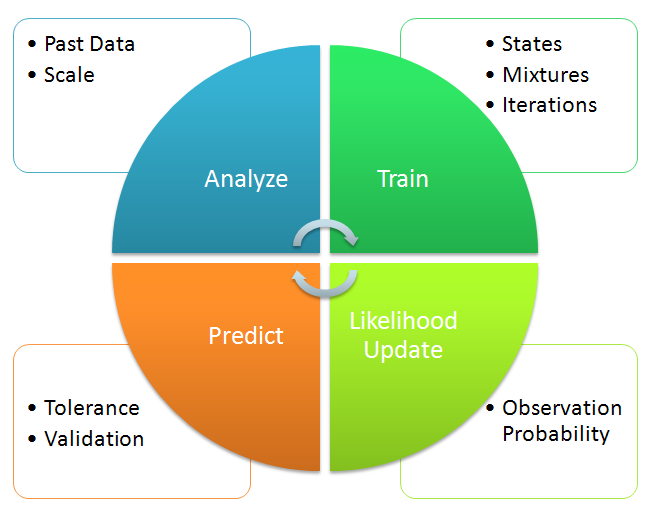
\includegraphics[scale=0.35]{ApproachOverview.png}}
\caption{Process Overview} \label{fig:appoverview}
\end{figure}


\subsection{Stock Data Retrieval} \label{sec:data}
There are a number of sources of stock and financial data on web including Google Finance and Yahoo! Finance. In the
specific case of \textbf{FTSE Index}, it seems that Google Finance does not provide the required data format as
required. As an alternative, Yahoo! Finance was used to load and store the stock data from $1984$. In the application
developed for this project, an interface is included to use when needed to load the data beforehand using the
algorithms for training and prediction.

\subsection{Statistical Report} \label{sec:stats}
Taking a very brief look at the history of FTSE Index stock data, it reveals that this stock index has gone through a
very vast range of changes over time since $1984$. This fact is important as the problem is being solved using some
techniques to first \textit{train an HMM} for which the historical data is being used. Intuitively, one can say that
the changes of stock trends during the $90$'s would not somehow be relevant, constructive, or informative of the recent
stock trends in the past couple of years. To create a better impression, we tried to do some simple analysis on the
historical data since $1984$. Figure \ref{fig:ftse-mean} shows the compared mean values of the four indices; namely, open,
high, low, and close; during different ranges of time.

\begin{figure}[h]
\centering
\setlength\fboxsep{0.1pt}
\setlength\fboxrule{0.7pt}
\fbox{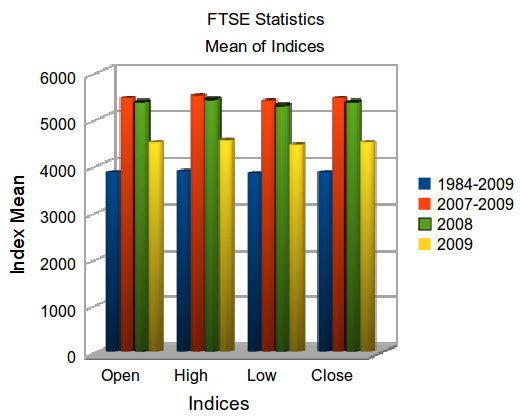
\includegraphics[scale=0.6]{ftse-mean.png}}
\caption{FTSE Stock Indices Mean Values over time periods} \label{fig:ftse-mean}
\end{figure}

As in Figure \ref{fig:ftse-mean}, we can say that whereas the period of $2007$ to $2009$ has been the most
flourishing period in FTSE Index, it is obvious that it has dropped drastically since the beginning of $2009$. Thus,
one conclusion might be that training an HMM with historical data from the period $2009-2009$ would not be wise to be
used for the prediction of the values in year $2009$. On the other hand, Figure \ref{fig:ftse-std} shows the standard
deviation of the indices for the same periods.

\begin{figure}[h]
\centering
\setlength\fboxsep{0.1pt}
\setlength\fboxrule{0.7pt}
\fbox{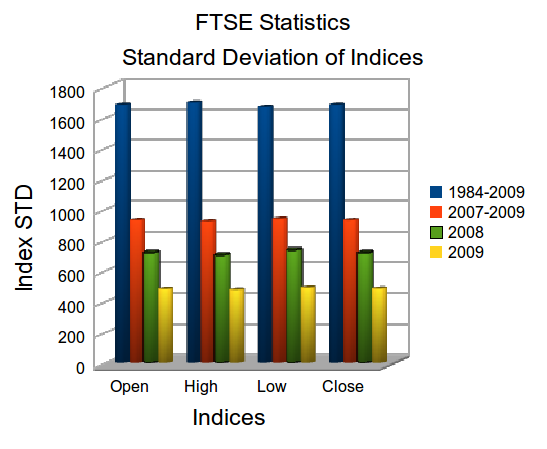
\includegraphics[scale=0.6]{ftse-std.png}}
\caption{Process Overview} \label{fig:ftse-std}
\end{figure}

With reinforcement, Figure \ref{fig:ftse-std} somehow shows that although as time passes, FTSE Index fails to be more
promising, the deviation from mean values are less likely to happen; i.e. index values tend to obey the most likely the
same behavior in time that could be highly useful in prediction. Thus, we tried to use the latest stock data history to
train and predict the values for the current year.

\subsection{Data Scaling} \label{sec:scale}
As the statistical report shows in Section \ref{sec:stats}, there are times that the data could be skewed unequally and
unevenly over time. Thus, an approach before starting to train the HMM would be to scale the data values to a specific
range such as $[-1, 1]$ using the maximum and minimum values in the range that the algorithms are taken effective.
Scaling is also proposed and implemented in \cite{hassan:hmm_stock_fuzzy}.

\subsection{HMM Training} \label{sec:train}
In this problem, there is a sequence of data over time with which we need to train an HMM; Problem (3) in Section
\ref{sec:hmm_probs}. To train an HMM matching a set of the sequence of stock index data as $\vec{O} = (open, high, low,
close)$, the following settings and considerations have been taken into account:
\begin{enumerate}
  \item \textbf{States:} in the experiments, we have $N = 4$; intuitively, it is denoting the stages in time that are
  allowed in different transitions in the HMM training.
  \item \textbf{Dimensions:} as a mixture of multivariate Gaussian is utilized in this problem, we have $D = 4$ as the
  observation vector for each stock date is as $(open, low, high, close)$.
  \item \textbf{Mixtures:} \cite{hassan:hmm_stock} proposes to have $M = 3$.
  \item \textbf{Left-Right Delta:} experimentally, we have tried $\Delta = 1$ and $\Delta = 3$.
  \item \textbf{Prior Probability:} Adhering to the left-right HMM, we have $\pi = (1, 0, 0, 0)$.
  \item \textbf{HMM Training:} According to \cite{hassan:hmm_stock,rabiner:hmm}, we need to use \textbf{Baum-Welch
  Learning Algorithm} to train the HMM. Baum-Welch training algorithms does its job based on a number of
  \textit{iterations} to tune and update the parameters of the model, namely the transition probability $B$.
\end{enumerate}

\subsection{Likelihood Update} \label{sec:likelihood}
In the path to prediction, first, there is a need to find the most similar day in stock market data for a specific day
so that it could be used to predict the following day's close value. To do so, first, we need to compute the
likelihood of previous days in the desired range. When having one day's stock data, it is straightforward to compute
the likelihood of that specific day from the HMM. This is Problem (1) in Section \ref{sec:hmm_probs} which is computed using
\textbf{Forward Backward Algorithm} proposed in \cite{rabiner:hmm,erwin:datamining,wiki:hmm}. Algorithm
\ref{alg:likelihood} overalls depicts the method to compute likelihoods.

\begin{algorithm}[h]
\caption{Likelihood Update Algorithm} \label{alg:likelihood}
\begin{algorithmic}[1]
\REQUIRE {Trained HMM $\lambda = (\pi, A, B)$}
\REQUIRE {Likelihood Update Start Date $start\_date$}
\REQUIRE {Likelihood Update Range $days$}
\STATE $date \gets start\_date$
\FOR {$i = 1$ to $days$}
\STATE $ O(open, high, low, close) \gets load(date) $
\STATE $ p \gets P(O|\lambda) $ \COMMENT {Forward Backward Algorithm}
\STATE $ persist(date, log10(p)) $
\STATE $ date \gets tomorrow(date) $
\ENDFOR
\end{algorithmic}
\end{algorithm}

\subsection{Prediction} \label{sec:pred}
When the likelihood probabilities of different days are computed, the last phase would be to predict some day's close
value as the target of this experiment. To do so, we introduce a parameter \textbf{likelihood tolerance} denoting the
similarity neighborhood that we can accept similar days to the previous day. Through using the likelihood tolerance, we
fetch a list of similar days to yesterday's stock data and then we try to find the best guess as the one that has the
highest likelihood of all. In this experiment, we used the likelihood tolerance value in range \boldmath{[0.001, 0.01]}
From this point, prediction is straightforward with calculating the difference of the similar day and yesterday's
values and then calculating tomorrow's close value. Algorithm \ref{alg:prediction} shows the overall pseudo-code used
for prediction. Along with prediction computation, we calculate also the \textbf{MAPE} (Mean Average Percentage
Error) measure.

\begin{algorithm}[h]
\caption{Prediction Algorithm} \label{alg:prediction}
\begin{algorithmic}[1]
\REQUIRE {Prediction Start Date $start\_date$}
\REQUIRE {Prediction Days $days$}
\REQUIRE {Likelihood Tolerate $tolerance$}
\STATE $ sum \gets 0 $
\STATE $ date \gets start\_date $
\FOR {$i = 1$ to $days$}
\STATE $ yesterday \gets yesterday(date) $
\STATE $ O_y \gets load(yesterday) $
\STATE $ O_a \gets load(date)$
\STATE $ likelihood_y \gets load\_likelihood(yesterday) $
\STATE $ similars_y \gets find(yesterday, likelihood_y, tolerance) $
\STATE $ most\_similar = find\_best\_guess(similars_y) $
\STATE $ tomorrow_{m\_s} \gets load(most\_similar.date) $
\STATE $ predicted\_close = O_y.close + (tomorrow_{m\_s}.close - most\_similar.close) $
\STATE $ sum \gets sum + \frac{|O_a.close - predicted\_close|}{O_a.close} $
\STATE $ date \gets tomorrow(date) $
\ENDFOR
\STATE $ MAPE \gets \frac{sum}{days} \times 100 $
\RETURN {Prediction Results + MAPE}
\end{algorithmic}
\end{algorithm}

\subsection{Validation} \label{sec:valid}
To validate this experiment, as we have an application developed for it, we easily load the data for the past desired
duration, then train the application for a period in $2009$ and try to predict the closing months of the year $2009$.
Accordingly, Figure \ref{fig:validation} shows the last three months of the year predicted values for FTSE Close Index
value.

\begin{figure*}[t]
\centering
\setlength\fboxsep{0.1pt}
\setlength\fboxrule{0.7pt}
\fbox{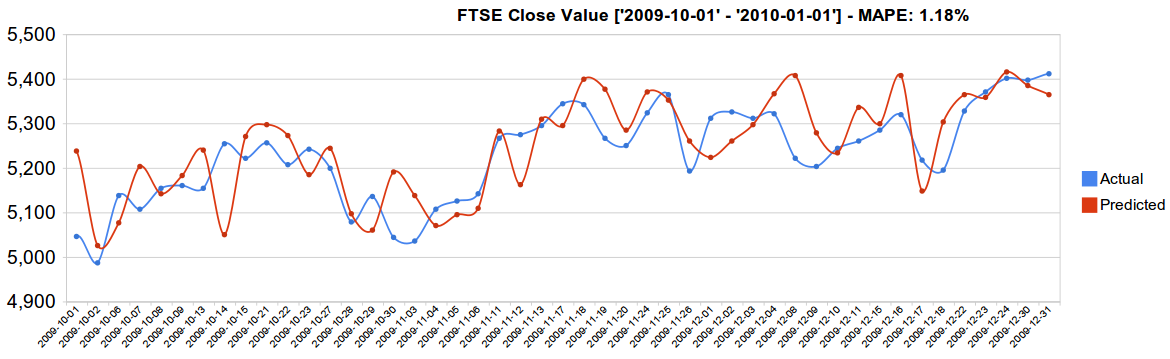
\includegraphics[scale=0.4]{ftse-validation.png}}
\caption{Predicted vs. Actual ``close'' values from $2009/10/01$ to $2010/01/01$ with $tolerance = 0.05$}
\label{fig:validation}
\end{figure*}

\section{Experiments and Results} \label{sec:results}
As an application is developed for this assignment, a sample result from the application is presented here. Figure
\ref{fig:res1} depicts a sample run from the application in which a prediction of $720$ days from $2008/01/01$ to
$2010/01/01$ is done using an HMM with settings in Table \ref{tbl:res1}.

\begin{table}[h]
\centering
\begin{tabular}{l l r}
\textbf{Parameter} & \textbf{Description} & \textbf{Value} \\ \thickhline
$N$ & Number of states in HMM & $4$ \\ \hline
$M$ & Number of Multivariate Gaussians & $3$ \\ \hline
$D$ & The dimension of each distribution & $4$ \\ \hline
$\Delta$ & The left-right HMM parameter & $3$ \\ \hline
$tolerance$ & The Likelihood Tolerance & $0.01$ \\ \hline
\end{tabular}
\caption{Sample settings for the run} \label{tbl:res1}
\end{table}

\begin{figure*}[t]
\centering
\setlength\fboxsep{0.1pt}
\setlength\fboxrule{0.7pt}
\fbox{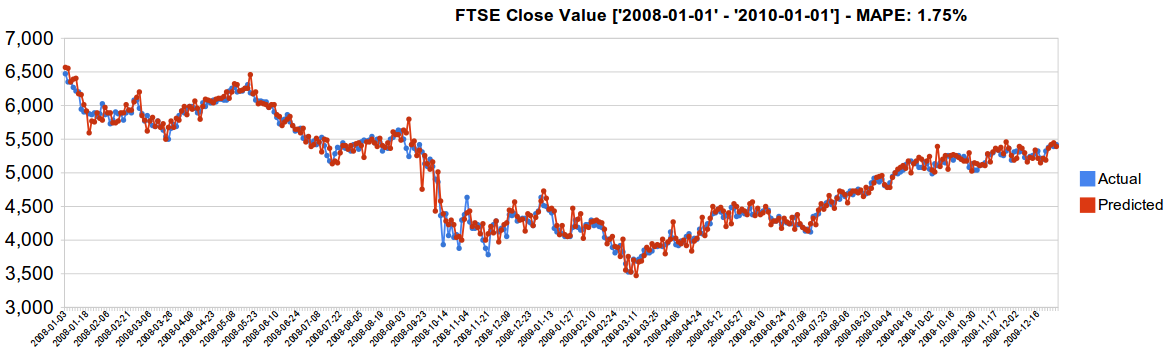
\includegraphics[scale=0.4]{2008-01-01___2010-01-01___720.png}}
\caption{Predicted vs. Actual ``close'' values from $2008/01/01$ to $2010/01/01$} \label{fig:res1}
\end{figure*}

\section{Implementation} \label{sec:impl}

\subsection{JAHMM}
As HMM is used in this implementation, there is a need to have an API for HMM operations. Among different
implementations, we chose to use \textbf{JAHMM} Java library, \cite{jahmm}.

\subsubsection{HMM Algorithms}
HMM-related algorithms such as Baum-Welch and Forward Backward we are provided with JAHMM package and no further
implementation was done in this regard.

\subsection{Extensions to JAHMM}

\subsubsection{Mixture of Multivariate Gaussian Distribution}
As JAHMM does not provide an implementation for the mixture of multivariate Gaussian distribution, one was developed to
be used in the experiments. The classes \textit{MultiGaussianMixtureDistribution},
\textit{OpdfMultiGaussianMixtureDistribution}, and \textit{OpdfMultiGaussianMixtureDistributionFactory} provide the
implementation.

\subsubsection{Left-Right HMM}
JAHMM does not implement the concept of a left-right HMM for which an implementation is given in our project. The class
$LeftRighHmm$ provides the implementation.

\subsection{Process Realization}
Briefly, the implementation project for this experiment takes advantage of Google Web Toolkit
(GWT)\footnote{\url{http://code.google.com/p/webtoolkit}} Version $2.0$ as its GUI layer and Spring
Framework\footnote{\url{http://www.springframework.org}} Version $3.0$ including Spring Core, Spring MVC, and Spring DAO
in different layers of the application. Additionally, MySQL\footnote{\url{http://www.mysql.com}} is used for the
back-end data storage.

\subsubsection{Data Retrieval}
Mainly, there are two classes, \textit{FTSEDownloader}, \textit{FtseJdbcManager} and \textit{FtseLikelihoodJdbcManager}, that
in charge of data retrieval requirements in the project including downloading the data from Yahoo! Finance, persisting the data,
retrieving different queries on FTSE data; generally implementing the data access layer for the FTSE data.

\subsubsection{FTSE Stock Service}
Generally, it has been tried to develop a simple single-point-of-action service layer for FTSE stock data services.
This service object implemented by class \textit{FtseStockService} provides the following interfaces:
\begin{enumerate}
  \item \textbf{HMM Training:} taking advantage of an instance \textit{HmmTrainer} provides an interface to train the required
  HMM in the experiment.
  \item \textbf{Likelihood Update:} that is done through an instance of \textit{FtseLikelihoodService}.
  \item \textbf{Prediction:} for which an object of \textit{FtsePredictor} is being used.
\end{enumerate}

\subsubsection{Web Interface}
All the client side implementation of the Web interface of the application is connected to the FTSE Stock Service layer
through GWT RPC mechanism and Spring MVC framework.

\subsubsection{Application Configuration}
Application configuration is done through Spring Container's XML configuration files. The main configuration file for
the application in in \textit{ftse-config.xml} and configurations required for MVC layer is done through
\textit{ftse-servlet.xml}. And, one required \textit{web.xml} initializes the application in a standard application
container such as Apache Tomcat\footnote{\url{http://tomcat.apache.org}}.

\subsubsection{Project Source}
This project is available under \textit{Apache License Version 2.0} in \cite{ftse}. Easy and complete instructions of
how to get the source and run the project is available at \cite{ftse:wiki}.

\subsection{Application Architecture}
It has been tried to develop a simple but extensible application for the purposes in this assignment. Very briefly,
Figure \ref{fig:apparch} depicts the overall architecture that has been adopted in the development of the application.

\begin{figure}[h]
\centering
\setlength\fboxsep{0.1pt}
\setlength\fboxrule{0.7pt}
\fbox{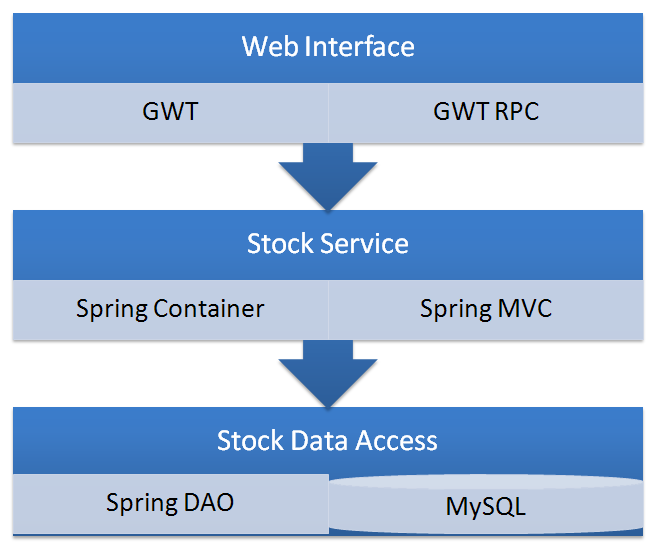
\includegraphics[scale=0.35]{AppArchitecture.png}}
\caption{Application Architecture Overview} \label{fig:apparch}
\end{figure}

\section{Future Works} \label{sec:future}
As it is revealing, we have been successful rough estimation of the future data required in the project. Though, the
quality of ``\textbf{preciseness}'' becomes more significant as the sensitiveness of the data rises. Thus, regarding
the work that has been done, for future, one of the ideas to apply to gain better quality is to consider
\textit{weighted} ranking of the most similar past data in search for the likelihood tolerance. Intuitively, it will
somehow try to control the deviation from the actual values that are seen over time. Additionally, further boundary
checks could be applied to the predicted data to prevent undesired deviations in the predictions

Another idea could be proposed as ``continuous training''; as opposed to the current situation in which a period of
time is considered and for that an amount of data is located and used to train an HMM. Then the trained HMM is used for
prediction purposes. However, a better idea is to somehow \textbf{persist} the trained HMM and over time try to
optimize and tune the HMM according to the latest data that emerge in time. This way, intuitively, we would be trying
to optimize and improve the HMM over time without losing the trained HMM from the past.

\section{Acknowledgments} \label{sec:ack}
We would like to express our thanks to Hossein Rahmani with whom we had some discussions on the problem; even though
they were brief yet so intuitive.

\bibliographystyle{plain}
\bibliography{references}
\end{document}
